\section{Aufgabe 2.1: Clientseitige Formularvalidierung}
\begin{frame}{Aufgabe 2.1}
\begin{center}
Implementierung einer clientseitigen Formularvalidierung mithilfe von JavaScript (innerhalb der HTML-Datei):\\
~\\~\\
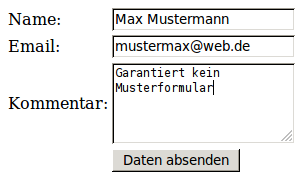
\includegraphics[width = 120px]{../A1/src/formvali.png}
\\
Betrachtet werden die für die Aufgabe relevanten $\langle${\bf form}$\rangle$ - und $\langle${\bf script}$\rangle$ -Blöcke:
\end{center}
\end{frame}


\tiny{\begin{lstlisting}[language = HTML,
				   mathescape = true, 
                   morekeywords = {onsubmit, onclick, this, return}, 
                   numbers = left, 
                   numbersep = 3pt]
 <form name = "vali" method = "post" action = "aufgabe2_1.html"
 onsubmit = "return$~$validate(this);">
<table border= "0" cellpadding= "0" cellspacing= "4">
 <tr>
  <td align = "left">Name:</td>
  <td align = "left">
  <input type = "text" name = "nameTextField" size = "20"></td>
 </tr>
 <tr>
  <td align = "left">Email:</td>
  <td align = "left">
  <input type = "text" name = "eMailTextField" size = "20"></td>
 </tr>
 <tr>
  <td align = "left">Kommentar:</td>
  <td align = "left">
  <textarea name = "commentTextArea" rows = "4" cols = "15">
  </textarea></td>
 </tr>
 <tr>
  <td align = "left"></td>
  <td align = "left">
  <input type = "button" value = "Daten$~$absenden" name = "validateButton" 
   onclick = "validate(this);"></td>
 </tr>
</table>
</form>
\end{lstlisting}}

\begin{frame}{Anmerkungen zum $\langle$form$\rangle$ - Block}
\normalsize{
\begin{itemize}
\item Bevor die Daten abgeschickt werden können, muss {\bf onsubmit = $"true"$} sein.
\item Durch einen Klick auf den Button {\bf Daten absenden} überprüft die Methode {\it validate()}, ob alle Angaben korrekt sind (true) oder nicht (false).
\end{itemize}}
\end{frame}

\tiny{
\begin{lstlisting}[language = JavaScript,
				   mathescape = true, 
                   numbers = left, 
                   numbersep = 3pt]
<script language = "JavaScript">
<!--
function validate() {
  var name        = document.vali.nameTextField.value;
  var eMail       = document.vali.eMailTextField.value;
  var comment     = document.vali.commentTextArea.value;
  var regExpName  = /([a-zA-Z]{2,})\s([a-zA-Z]{2,})/i;
  var regExpMail  = /^(\w[\w.]{2,}@)(\w{2,}.)*([a-zA-Z]{3,}\.[a-zA-Z]{2,4})/$\$$i;
	
  if(name != "" && eMail != "" && comment != "") {
	 if(regExpMail.test("" + eMail) == false) {
		 alert("Ungueltige Emailadresse.");
		 return false;
	 }
	 else if(regExpName.test(name) == false) {
		 alert("Ungueltiger$~$Name.$~$Namen$~$in$~$der$~$Form$~$\n$~$
		 Vorname<Leerzeichen>Nachname$~$angeben.");
	 }	
	 else { 
		 alert("Daten$~$wurden$~$erfolgreich$~$abgeschickt.$~$\n$~$Ihre$~$Daten:$~$\n$~$
		 Name:$~$" + name + "\n$~$Email:$~$" + eMail + "\n$~$Kommentar:$~$" 
		 + comment);	
		 return true;	
	 }
  }
  else {
	 alert("Es$~$wurden$~$noch$~$nicht$~$alle$~$Felder$~$ausgefuellt.");
	 return false;
  }
}; -->
</script>
\end{lstlisting}}

\begin{frame}{Anmerkungen zum $\langle$script$\rangle$ - Block}
\small{
\begin{itemize}
\item {\it validate()} überprüft mittels regulärer Ausdrücke\\ (Zeile 7 u. 8) die Angaben auf Korrektheit:
	\begin{itemize}
	\item {\bf Name} hat die Form Vorname$\langle$Leerzeichen$\rangle$Nachname
	\item {\bf Emailadresse} hat die Form \newline [min. 3 Zeichen ]@[min. 3 Zeichen].[2 - 4 Buchstaben]
	\end{itemize}
\item Bei einer ungültigen Eingabe oder nicht ausgefüllten Feldern erscheint eine Fehlermeldung in Form einer Alert-Box .
\item Sind alle Angaben korrekt, erscheint eine Alert-Box mit den angegebenen Daten.
\end{itemize}}
\end{frame}
